\chapter{Análisis de los datos}

Este capı́tulo está destinado al estudio y tratamiendo de los datos. Se encuentra dividido en 5 secciones. La primera denominada Introducción al problema 5.1, nos habla sobre porque es importante tratar los datos de los sensores en el desarrollo de este proyecto. La segunda sección llamada Cálculo de la velocidad 5.2, describe como se obtiene la velocidad a partir de la aceleración. La tercera sección denominada Calibración de los sensores 5.3, comenta tres técnicas diferentes para conseguir eliminar la componente gravitacional de la aceleración. La sección Pruebas de calibración 5.4, pone las técnicas descritas en el apartado anterior a prueba. Finalmente, la sección Eliminación de ruido mecánico 5.5, describe un método para eliminar ruido de los sensores.

\section{Introducción al problema}

Se supone el siguiente escenario. El usuario llevará un dispositivo wearable atado a la muñeca y se debe calcular la potencia desarrollada por el usuario en base a los datos que puede aportar el werable. Como se ha presentado en el capítulo 1 de esta memoria, se deberá calcular la velocidad y la fuerza con el fin de obtener la potencia.
\\
\\
Para calcular la velocidad se procederá a integrar la aceleración y para calcular la fuerza tambien se deberá utilizar la aceleración. Por lo que para el correcto funcionamiento de la aplicación y para que sea lo más precisa posible, se debe calcular con la máxima fiabilidad la aceleración.

\section{Calculo de la velocidad}

En esta sección se va a proceder a calcular la velocidad utilizando la integración matemática. Por lo que previamente, se va a definir la aceleración.
\\
La aceleración se define como la variación de la velocidad por unidad de tiempo. Viene representada por:
\\
\[a = \frac{dv}{dt}\]
\\
Cuando la aceleración no es constante aparece una nueva magnitud denominada '\textit{jerk}'. La constante jerk se define como la variación de aceleración respecto al tiempo. Viene representada por:
\\
\[j = \frac{da}{dt}\]
\\
Por lo que se deduce que jerk es la derivada de la aceleración. Para calcular la aceleración solo se debe integrar.
\\
\[da=j*dt\]
\\
\[\int_{a_{0}}^{a}da=\int_{0}^{\partial t}j*dt\]
\\
\[a - a_{0} = j *\partial t\]
\\
\[a = a_{0} + j *\partial t\]
\\
\\
Por otro lado se tiene que la aceleración es la derivada de la velocidad, por lo que que:
\\
\[a = \frac{dv}{dt}\]
\\
\[dv=a*dt\]
\\
\[dv=a_{0} + j *\partial t\*dt\]
\\
\[\int_{v_{0}}^{v}dv=\int_{0}^{\partial t}(a_{0}*jt)dt\]
\\
\[v-v_{0}=a_{0}*\partial t+\frac{1}{2} j \partial t^{2}\]
\\
Teniendo así finalmente la ecuación de la velocidad:
\\
\textbf{
\[v=v_{0}+a_{0}*\partial t+\frac{1}{2} j \partial t^{2}\]}
\\
\\
Una manera de calcular la velocidad es la integral debajo de la curva, donde la integración es la suma de las áreas de longitud mínima.

\begin{figure}[h]
	\centering
	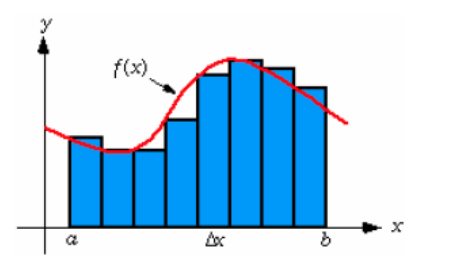
\includegraphics[scale=0.7]{imagenes/velocidad.png}
	\caption{Señal del acelerómetro \cite{nxp}.}
	\label{Calculo velocidad}
\end{figure}

Donde:
\[\int_{a}^{b}f(x) dx=\lim_{n\rightarrow \infty }\sum_{i=1}^{n}f(x_{i})\partial x\]
\\
\[\partial x = \frac{b-a}{n}\]
\\
\[Area_{n} = Muestra_{n} +\frac{\left | Muestra_{n}-Muestra_{n-1} \right |}{2} * T\]
\\
\\
\section{Calibración de los sensores}

Los sensores aportan datos con diferentes ruidos y fluctuaciones como se pudo ver en la sección 2.2 de esta memoria. En este apartado se va a tratar de compensar y calibrar el acelerómetro.
\\
La salida del acelerómetro por norma general varía entre 0V y Vdd, y dicha salida es interpretada por un comparador (A/D). Por lo tanto el valor 0 de la aceleración deberá corresponder con Vdd/2.
\\
Un acelerómetro por defecto esta sometido a la fuerza de la gravedad, así que por defecto la gravedad sobre el eje 'Y' será (situando el sistema de coordenadas sobre el eje de la tierra):
\\
\[g = 9.81 m/s^{2}\]
\\
Por lo que será necesario compensar la aceleración con el fin de eliminar este valor, para ello se van a comparar y aplicar tres técnicas con el fin de averiguar cuál nos ofrece unos datos más precisos.

\subsection{Compensación gravitatoria utilizando Sensor Fusion}

\textbf{Sensor Fusion} se define como el uso de varios sensores con el fin de incrementar la precisión de las mediciones.
\\
\\
En este caso, se va a utilizar el algoritmo de Madgwick, el cual hace uso del acelerómetro, giroscopio y magnetómetro para calcular de manera computacionalmente eficiente la orientación del dispositivo IMU\cite{madgwick}.
\\
El algoritmo produce una representación de la orientación en forma de quaternion\cite{quaternion}. Para ello calcula la rotación que alinea la rotación del dispositivo con la con la de la tierra utilizando un algoritmo de gradiente descendiente. Se puede encontrar el algoritmo en el siguiente repositorio, bajo licencia GNU \cite{algoritmo}.
\\
La baja carga computacional de este algoritmo y su capacidad de operar a frecuencias de muestreo bajas, lo hacen ideal para medir el movimiento en dispositivos wearable.
\\
\\
Una vez se ha obtenido la orientación del dispositivo se puede eliminar la componente gravitatoria de cada eje de coordenadas de una manera mucho más precisa, de la siguiente manera:
\\
\[quaternion = q0,q1,q2,q3\]
\\
\[aceleracion_x = raw\_acceleracion_x - 2 * (q1 * q3 - q0 * q2);\]
\\
\[aceleracion_y = raw\_acceleracion_y - 2 * (q0 * q1 + q2 * q3);\]
\\
\[aceleracion_z = raw\_acceleracion_z - q0 * q0 - q1 * q1 - q2 * q2 + q3 * q3;\]

\subsection{Filtro de paso bajo}

Un filtro de paso bajo es un filtro electrónico que deja pasar señales de frecuencia baja y reduce la amplitud de las señales con frecuencias más altas que la frecuencia de corte.
\\
\\
Utilizando un filtro de paso bajo se puede aislar la fuerza de la gravedad de la aceleración y por lo tanto corregir el valor real de la aceleración.
\\
\\
Antes de aplicar el filtro, se debe denfinir una constante alfa como:
\\
\[alpha = t / (t + dT)\]
\\
Siendo t la constante de tiempo del filtro y dT la tasa de llegada de datos.
\\
\\
\[gravity_0 = alpha * gravity_0 + (1 - alpha) * aceleracion_x;\]

\[gravity_1 = alpha * gravity_1 + (1 - alpha) * aceleracion_y;\]

\[gravity_2 = alpha * gravity[2] + (1 - alpha) * aceleracion_z;\]
\\
\\
Eliminando así la componente gravitatoria de cada eje:
\\
\\
\[aceleracion_x = raw\_acceleracion_x - gravity_0\]

\[aceleracion_y = raw\_acceleracion_y - gravity_1\]

\[aceleracion_z = raw\_acceleracion_z - gravity_2\]

\subsection{Aceleración Lineal}

La API SensorManager provee de un tipo de sensor denominado TYPE\_LINEAR\_ACCELERATION comentado en la sección del 2.3. Conceptualmente el sensor porporciona la aceleración siguiendo la siguiente norma:
\\\\
\[aceleracion\_lineal = aceleracion - gravedad\]
\\
Se debe tener en cuenta que este sensor siempre presenta un offset(compensación), por lo que una rutina de calibración deberá ser necesaria, leyendo y eliminando el valor offset de los datos del sensor.

\section{Pruebas de calibración}

Se va a mostrar como se comportan los diferentes sensores en condiciones de parada y de movimiento (todos bajo las mismas circunstancias), durante un intervalo de 10 y 30 segundos respectivamente. Y se podrá observar el calculo de la velocidad obtenida en base a los distintos datos resultantes.

\subsection{Condición de parada}

Con una circunstancia de movimiento 0 del wearable. (Por lo tanto la aceleración ideal deberá ser 0). Se toman muestras para cada método:
\subsubsection{Validación compensación gravitatoria utilizando Sensor Fusion}

\begin{figure}[H]
	\centering
	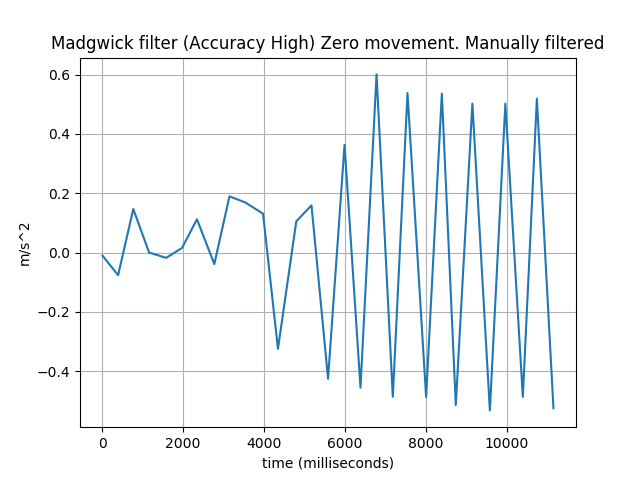
\includegraphics[scale=0.5]{imagenes/madwickZero.png}
	\caption{Compensación de la gravedad por medio del algoritmo de Madgwick (sin movimiento).}
	\label{Movimiento cero Madgwick}
\end{figure}


\begin{figure}[H]
	\centering
	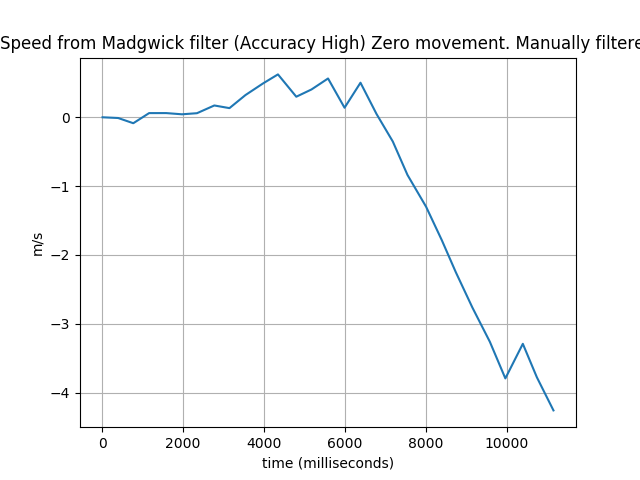
\includegraphics[scale=0.5]{imagenes/madwickZeroSpeed.png}
	\caption{Velocidad calculada de la aceleración por medio del algoritmo de Madgwick (sin movimiento).}
	\label{Velocidad cero Madgwick}
\end{figure}
\noindent
Como se puede ver, la aceleración varía rápidamente y su amplitud va aumentando segundo a segundo, lejos de ser estable y precisa.

\subsubsection{Validación filtro de paso bajo}

\begin{figure}[H]
	\centering
	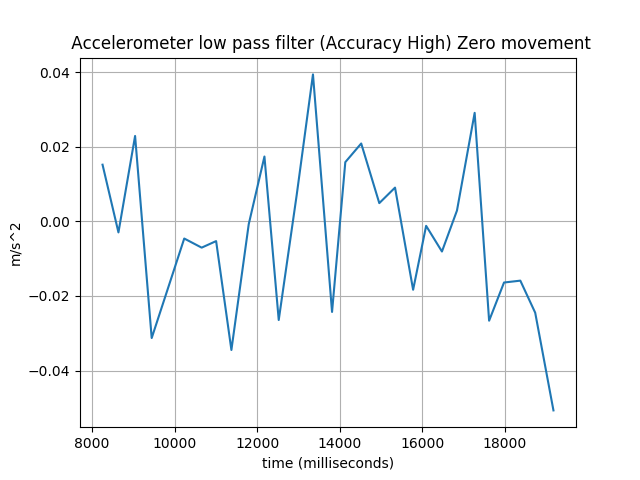
\includegraphics[scale=0.5]{imagenes/lowpass0mov.png}
	\caption{Compensación de la gravedad por medio de un filtro de paso bajo (sin movimiento).}
	\label{Movimiento cero filtro paso bajo}
\end{figure}

\begin{figure}[H]
	\centering
	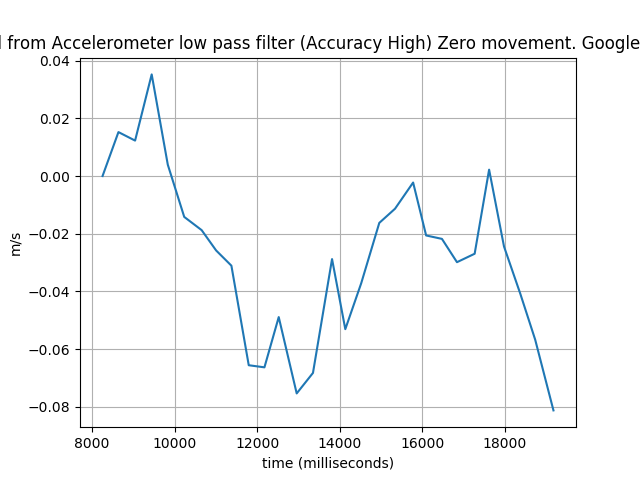
\includegraphics[scale=0.5]{imagenes/lowpass0movspeed.png}
	\caption{Velocidad calculada de la aceleración por medio de un filtro de paso bajo (sin movimiento).}
	\label{Velocidad cero filtro paso bajo}
\end{figure}
\noindent
Se puede observar como la aceleración varía de considerablemente menos que en el método anterior, teniendo una reducción de un -93,33\% en el valor máximo. Donde la diferencia es más notoria es en el cálculo de la velocidad, habiendo una diferencia a los 11000 ms de 4 m/s\^2 a -0,02 m/s\^2.


\subsubsection{Validación aceleración lineal}

\begin{figure}[H]
	\centering
	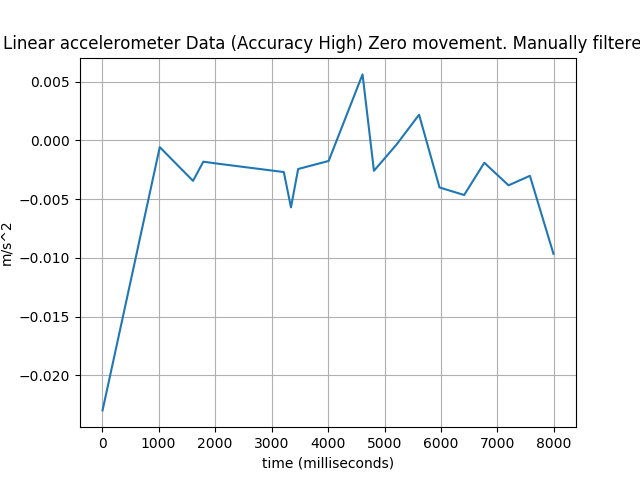
\includegraphics[scale=0.5]{imagenes/linearGoogleZero.png}
	\caption{Compensación de la gravedad por medio de la aceleración lineal (API) (sin movimiento).}
	\label{Movimiento cero aceleracion lineal}
\end{figure}

\begin{figure}[H]
	\centering
	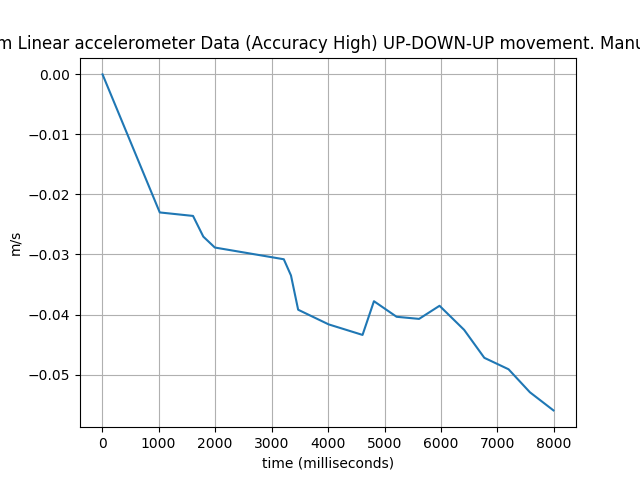
\includegraphics[scale=0.5]{imagenes/linearGoogleZeroSpeed.png}
	\caption{Velocidad calculada de la aceleración lineal (API) (sin movimiento).}
	\label{Velocidad cero aceleracion lineal}
\end{figure}
\noindent
En este caso, se aprecia como la aceleración máxima varía en un -82,61\% con respecto al filtro de paso bajo.
\\
\\
Su funcionamiento en líneas generales es muy parecido al del filtro de paso bajo.

\subsection{Condición de movimiento}

Esta vez se realizarán las pruebas en base al siguiente escenario. Circunstancia de movimiento de 60 cm en total a lo largo del eje Y (+30 cm y -30cm) del wearable y 30 segundos de tiempo de muestreo. Quedando el wearable apoyado sobre una superficie plana al final de la medición. Se debe tener en cuenta que la aceleración máxima producida es de 0,15m/s\^2.\\\\ Tomamos muestras para cada método:

\subsubsection{Validación compensación gravitatoria utilizando Sensor Fusion}

\begin{figure}[H]
	\centering
	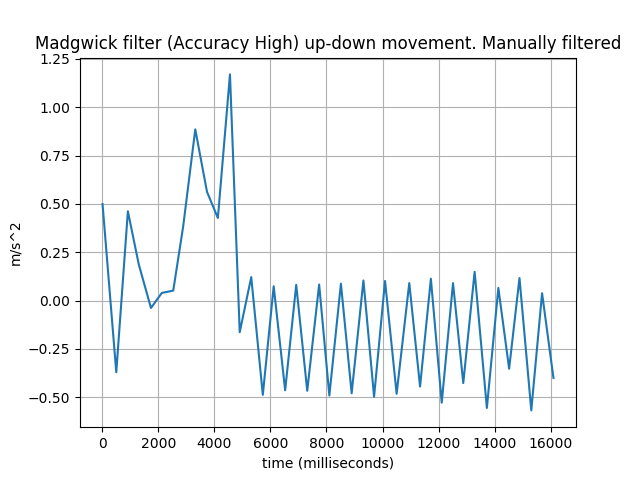
\includegraphics[scale=0.5]{imagenes/madwickup-down.png}
	\caption{Compensación de la gravedad por medio del algoritmo de Madgwick (con movimiento vertical).}
	\label{Movimiento vertical Madgwick}
\end{figure}


\begin{figure}[H]
	\centering
	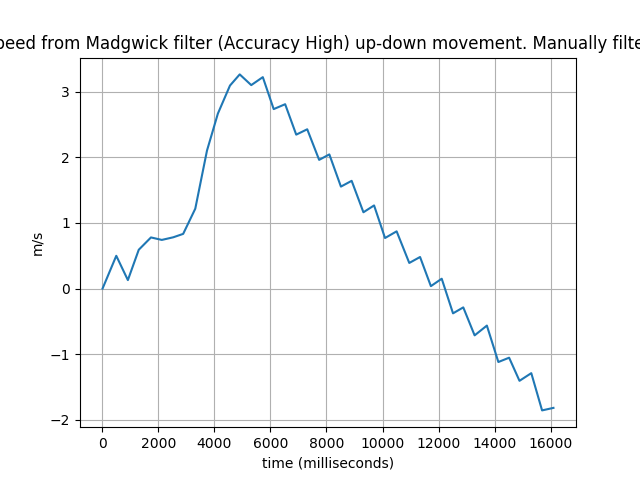
\includegraphics[scale=0.5]{imagenes/madwickup-downSpeed.png}
	\caption{Velocidad calculada de la aceleración por medio del algoritmo de Madgwick (con movimiento vertical).}
	\label{Velocidad vertical Madgwick}
\end{figure}
\noindent
Como se puede apreciar, la aceleración no es nada estable, sobre todo cuando se encuentra en condición de parada. Aumentando la amplitud de la señal en función del tiempo.

\subsubsection{Validación filtro de paso bajo}

\begin{figure}[H]
	\centering
	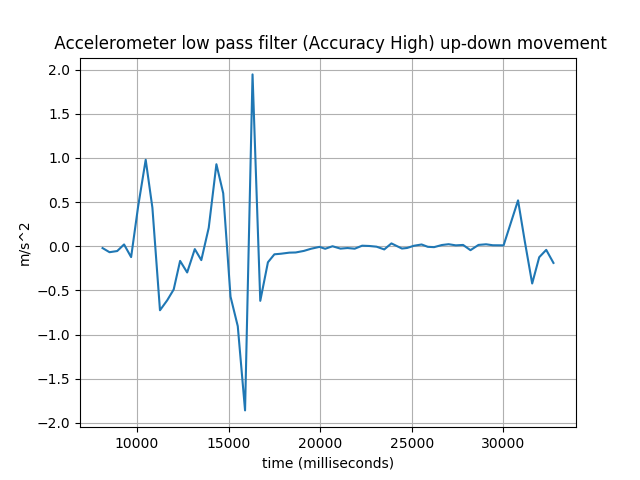
\includegraphics[scale=0.5]{imagenes/lowpassUpmov.png}
	\caption{Compensación de la gravedad por medio de un filtro de paso bajo (con movimiento vertical).}
	\label{Movimiento vertical filtro paso bajo}
\end{figure}

\begin{figure}[H]
	\centering
	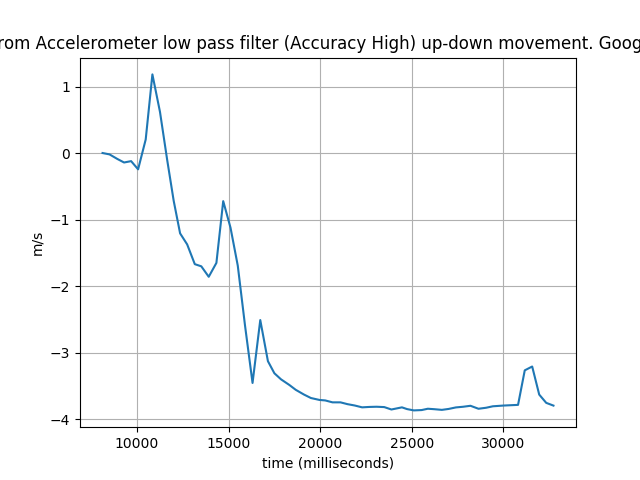
\includegraphics[scale=0.5]{imagenes/lowpassUpmovspeed.png}
	\caption{Velocidad calculada de la aceleración por medio de un filtro de paso bajo (con movimiento vertical).}
	\label{Velocidad vertical filtro paso bajo}
\end{figure}
\noindent
Se puede ver como la aceleración esta vez no flúctua cuando se encuentra en condición de parada, monitorizando correctamente cuando se encuentra en movimiento el dispositivo. Sin embargo, se aprecia como la aceleración en movimiento alcanza valores sustancialmente elevados y altos, no ajustados a la aceleración real.


\subsubsection{Validación aceleración lineal}

\begin{figure}[H]
	\centering
	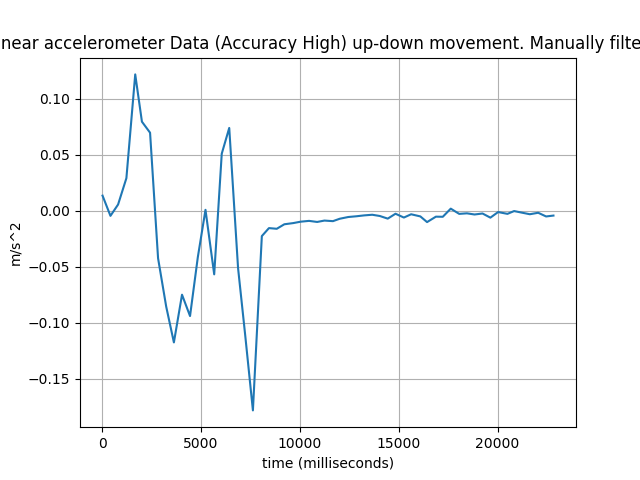
\includegraphics[scale=0.5]{imagenes/linearGoogleup-down.png}
	\caption{Compensación de la gravedad por medio de la aceleración lineal (API) (con movimiento vertical).}
	\label{Movimiento vertical aceleracion lineal}
\end{figure}

\begin{figure}[H]
	\centering
	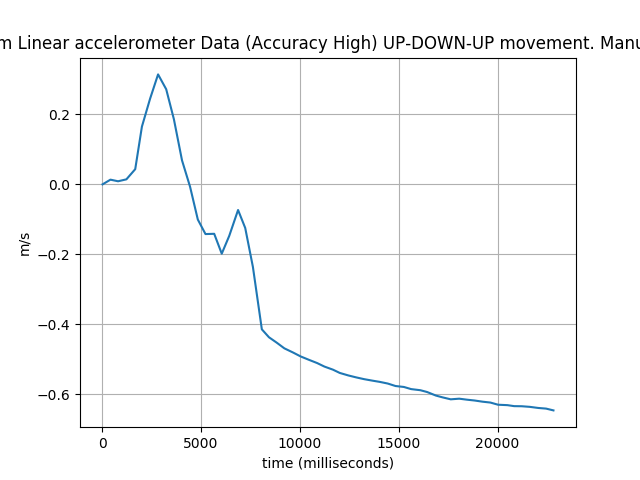
\includegraphics[scale=0.5]{imagenes/linearGoogleup-downSpeed.png}
	\caption{Velocidad calculada de la aceleración lineal (API) (con movimiento vertical).}
	\label{Velocidad vertical aceleracion lineal}
\end{figure}
\noindent
En este caso, la aceleración sí varía entre unos baremos reales, ajustándose más a los valores reales que el resto de métodos. Por lo que a priori parece el método más adecuado para utilizar en el sistema.

\section{Eliminación de ruido mecánico}

Una vez se ha eliminado la componente gravitatoria de los datos, aún cuando el wearable se encuentra en condición de parada, el acelerómetro produce valores inestables.
\\
\\
Por lo que es necesario construir una ventana de discriminación con el fin de considerar los valores que son ruido y los valores que representan aceleración real. De esta manera se mejora la precisión de la aceleración y consecuentemente de la velocidad calculada.
\\
\begin{figure}[H]
	\centering
	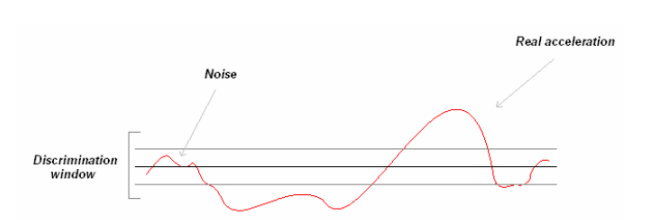
\includegraphics[scale=0.5]{imagenes/ventana.png}
	\caption{Ventana de discriminación \cite{nxp}.}
	\label{Ventana de discriminación}
\end{figure}
